\documentclass[../main.tex]{subfiles}

\begin{document}
	 \section{Die Legalisierung}
	 
	 \subsection{Das Konzept}
	 Für eine mögliche Legalisierung existieren viele Ansätze, wie weit eine Legalisierung gehen kann.
	 Eine Legalisierung bedeutet nicht, dass Cannabis ohne Einschränkungen für alle Menschen erlaubt wird.
	 Zurzeit sind es drei Länder, die Cannabis legalisiert haben.
	 Die Länder Südafrika, Uruguay und Kanada haben die Legalisierung mit verschiedenen Ansätzen und Einschränkungen durchgesetzt.
	 Georgien wird in dieser Arbeit nicht zu den Ländern mit einer Legalisierung gezählt, da zwar der Besitz und Konsum legal ist, jedoch der Anbau und Handel illegal bleibt. 
	 In Georgien gibt es für die Konsumenten keinen legalen Weg Cannabis zu besitzen.
	 
	 \paragraph{Südafrika}
	 Im Jahr 2018 entscheid das Verfassungsgericht Südafrikas, dass Cannabis für den Eigengebrauch komplett legalisiert werden sollte \cite{zacc}. 
	 Durch dieses Gerichtsurteil wurde gezielt nur der private Konsum und der Anbau kleiner Mengen legalisiert. 
	 In der Öffentlichkeit herrscht immer noch ein striktes Konsumverbot. 
	 Der Handel mit Cannabis und Cannabisprodukten bleibt weiterhin verboten und wird mit hohen Strafen bestraft. 
	 Damit werden alle Endkonsumenten entlastet, jedoch kann der südafrikanische Staat wirtschaftlich nur sehr wenig von der Legalisierung profitieren. 
	 Die Durchsetzungskosten der Polizei und Justiz fallen zwar weg, jedoch bleiben mögliche Steuereinnahmen komplett weg.
	 Für Touristen gibt es keinen Weg, Cannabis zu konsumieren, da kein legaler Cannabismarkt unter südafrikanischer Gesetzeslage existieren kann.
	 Das Fehlen des Marktes lässt einen Teil des Schwarzmarktes bestehen.
	 
	 \paragraph{Uruguay}
	 Uruguay ist das erste Land, das Cannabis für die Bevölkerung legalisiert hat.
	 Die Legalisierung von Cannabis in Uruguay erfolgt unter strenger staatlicher Kontrolle \cite{fijnaut}. 
	 Bürger können monatlich maximal 40 Gramm Cannabis in Apotheken beziehen oder ihr eigenes Cannabis in Cannabis Social Clubs anbauen.
	 Der Eigenanbau ist unter der Einschränkung erlaubt, dass man maximal 40 Gramm aus der Ernte gewinnen darf.
	 Konsumenten werden in staatlichen Registern registriert und der Handel wird staatlich streng kontrolliert.
	 Für Ausländer gibt es jedoch keine Möglichkeit Cannabis zu erwerben, da der staatliche Verkauf nur für volljährige Bürger vorgesehen ist.
	 Diese Methode löst einen Teil des Schwarzmarktes auf, jedoch können sich Anreize bilden, dennoch auf den Schwarzmarkt auszuweichen. 
	 Touristen werden dennoch auf den Schwarzmarkt ausweichen, da ihnen keine andere Wahl bleibt.
	 Der Konsum in der Öffentlichkeit ist strikt verboten und steht unter Strafe.
	 	 
	 
	 \paragraph{Kanada}
	 Kanada ist das erste Land, das Cannabis mit einem marktwirtschaftlichen Ansatz legalisierte.
	 Die Einschränkungen können zwar je nach Provinz stark schwanken, jedoch kann man einige Trends erkennen.
	 Die meisten Provinzen erlauben den Cannabiskonsum ab 19 Jahren und erlauben den Konsum überall, wo auch das Rauchen von Tabak erlaubt ist.
	 In den meisten Provinzen existieren keine Limits für die Menge des persönlichen Besitzes.
	 Die Händler unterstehen einer Lizenzierungspflicht und werden nur indirekt eingeschränkt. 
	 Es herrscht ein komplettes Werbeverbot auf Cannabis und die Verpackung muss den Vorlagen entsprechen.
	 
	 
	 \paragraph{Ein mögliches Schweizer Modell}
	 Die in der Arbeit angesprochene Legalisierung soll den Anspruch der Verdrängung des Schwarzmarktes so weit wie möglich erfüllen.
	 Der marktwirtschaftliche Ansatz Kanadas eignet sich für die Erfüllung dieses Zieles.
	 Ein Nebenziel, gefährdete Gesellschaftsgruppen zu schützen, wird durch eine Legalisierung weiterhin gestärkt, da der Jugendschutz erst auf den legalen Markt einwirken kann.
	 Das potentielle Schweizer Konzept ist so aufgebaut, dass sowohl Konsum und Besitz als auch Handel und Anbau unter bestimmten Bedingungen legal ist.
	 Niemand soll am Markteintritt gehindert werden, solange er sich an die Rahmenbedingungen hält.
	 Ausser den unten genannten Einschränkungen soll die Ressourcenallokation dem freien Markt überlassen werden. 	 
	 
	 
	 \subsection{Preisniveau}
	 
	 Um ein angemessenes Preisniveau zu finden, muss man sich stets den Zielen der Legalisierung bewusst sein. 
	 Durch eine Legalisierung möchte man den Schwarzmarkt zerstören und die Konsumenten weitestgehend in diesen integrieren. 
	 Um dieses Ziel zu erreichen darf man den Preis nicht zu hoch ansetzen, da sonst die Konsumenten dennoch auf den Schwarzmarkt ausweichen würden.
	 Weil man nicht die gesamte Nachfrage der Bevölkerung erhöhen will, darf man den Preis auch nicht tiefer als das präsente Preisniveau ansetzen.
	 Das Ziel ist es, die Nachfrage stabil zu halten oder gar zu senken.
	 Durch die Legalisierung kann man ein leicht höheres Preisniveau anstreben und Teile des Schwarzmarktes zerstören. 
	 Das liegt daran, dass die Kunden bereit sind, einen höheren Preis zu bezahlen, da im Gegenzug Qualität und Quantität gesichert ist. 
	 Man kann einen Preis von etwa 11.50 CHF anstreben. 
	 Dadurch wird sich die Nachfrage leicht senken und es bleibt ein grösserer Spielraum für die Besteuerung übrig.\\
	 
	 \noindent
	 Den Schwarzmarkt komplett zu zerstören, ist nahezu unmöglich, da sich zwei Gegensätze gebildet haben.
	 Ökonomisch gesehen würde man den Preis dem freien Markt überlassen, politisch gesehen ist dies jedoch nicht möglich.
	 Ein Nachfrageanstieg ist nicht mit den Zielen der Viersäulenpolitik vereinbart.\\
	 
	 \noindent	
	 Bei einer Legalisierung ohne Einschränkungen würde der Preis sofort fallen, was einen Nachfrageanstieg zur Folge hätte.
	 Um dem Nachfrageanstieg entgegenzuwirken, kann der Staat anhand der Steuerlast auf Cannabis den Preis in die richtige Richtung lenken.
	 Die Händler würden eine allfällige Erhöhung der internen Kosten, resultierend aus der Besteuerung, direkt den Kunden abgeben.
	
	 
	 \subsection{Rechtslage \& Einschränkungen}
	 
	 \subsubsection{Cannabisgesetz}
	 Die Legalisierung kann nicht ohne Einschränkungen erfolgen und deswegen muss man ein neues Gesetz in Betracht ziehen.
	 Als Beispiel dienen Gesetze über den Umgang mit Tabak und Alkohol.
	 Der gesetzliche Umgang mit Alkohol und mit Tabak, zwei legalen psychoaktiven Substanzen wird in eigenen Gesetzen geregelt. 
	 Aus diesem Grund müsste man für Cannabis ein neues Gesetz mit Verordnungen erlassen, das die Herstellung, Einfuhr und Ausfuhr, Verkauf und Besteuerung regeln würde.	 
	 Im Cannabisgesetz werden alle in den folgenden Untersektionen genannten Einschränkungen weiter konkretisiert.
	 
	 \subsubsection{Besteuerung}
	 Eine Cannabissteuer muss schon auf der höchsten Stufe der Normenhierarchie geregelt werden. 
	 Die Rechtsgrundlage der Besteuerung wird der von Alkohol und Tabak gleichen, da es sich bei allen drei Produkten um psychoaktive Substanzen handelt.
	 Die besondere Verbrauchssteuer nach \texttt{Art. 131 Abs. 1 BV} muss so erweitert werden, dass der Bund diese auch auf Cannabis und dessen Produkte erheben kann.
	 Die Einnahmen der Verbrauchssteuern sollen in Prävention und Behandlung von Suchtproblemen aber auch in die vorhandenen Ausgleichskassen fliessen.
	 Mit der Erweiterung von \texttt{Art. 131 Abs. 3 BV} für Prävention und Therapie und \texttt{Art. 112 Abs. 5 BV} für die AHV und IV mit Cannabis, ist die Grundlage für eine Besteuerung geebnet.\\
	 
	 \noindent
	 Nähere Bestimmungen über die Besteuerung würden im neuen Cannabisgesetz festgelegt werden.
	 Es existieren viele Faktoren, die sich für eine Besteuerungsgrundlage eignen würden, jedoch bewies sich die Besteuerung nach absolutem Inhalt bereits zahlreich.
	 Tabak- und Alkoholprodukte werden nach gleichem Prinzip besteuert und tragen einen wesentlichen Teil der Deckung der Schäden bei.
	 Auch Ausgleichskassen wie die AHV oder IV werden durch die Steuerlast der Produkte teilfinanziert.
	 Eine Besteuerung nach absolutem THC Gehalt ist der gewichtsbasierten Besteuerung zu bevorzugen, da sich dann keine Anreize für die Hersteller ergeben, den THC Gehalt künstlich hochzuzüchten.
	 Eine höhere Besteuerung auf potenteres Cannabis sollte chronische Konsumenten abhalten, immer potenteres Cannabis zu konsumieren, das einen höheren Schaden verursacht. \\
	 
	 \noindent
	 Das Ausmass der gesamten Besteuerung wird im Kapitel \texttt{Legalisierung > Besteuerung} ermittelt.
	 
	 
	 \subsubsection{Jugendschutz}
	 In erster Linie dient der Jugendschutz dem Wohle der Kinder und Jugendliche, dass sie von den Risiken des Betäubungsmittelkonsums geschützt werden und ihre psychische und physische Entwicklung nicht beeinträchtigt wird. 
	 So wird bei Alkohol das Schutzalter von hartem Alkohol bei 18 Jahren festgelegt. 
	 Bei Cannabis würde man auch ein Schutzalter zwischen 18 - 20 Jahren anstreben. 
	 Dies ist sinnvoll, da die Gehirnentwicklung des Menschen bei ungefähr 20 Jahren weitgehend abgeschlossen ist. 
	 Zwar ist mit 18 Jahren die Hirnentwicklung noch nicht vollständig abgeschlossen, jedoch kann man annehmen, dass erwachsene Menschen ab diesem Alter mehr Eigenverantwortung übernehmen können. 
	 Es wäre kontraproduktiv, einem Teil der grössten Gruppe an Konsumenten den Zugang zum legalen Markt zu verweigern, da diese sonst auf den Schwarzmarkt ausweichen. \\
	 
	 \noindent
	 Der Grundgedanke des Jugendschutzes besteht zwar aus einem Abgabeverbot an Jugendliche, jedoch gelten auch die Massnahmen der Vier-Säulen-Politik auch für den Jugendschutz. 
	 Deswegen folgt als direkte Auswirkung, dass schon konsumierende Jugendliche Hilfe bei der Bewältigung ihrer Sucht zur Verfügung gestellt bekommen. 
	 Neben der Suchthilfe für chronische Konsumenten ist auch die Früherkennung und Intervention von grosser Bedeutung. 
	 Durch eine Legalisierung wird der Konsum nicht mehr stark stigmatisiert, sodass Bezugspersonen die Situationen frühzeitig erkennen und handeln können. 
	 Die Prävention erhalten alle Jugendliche, sodass Kinder und Jugendliche wichtige Kompetenzen erlernen, sich gegen den Konsum von Betäubungsmitteln zu stellen.  
	 
	 \subsubsection{Werbeeinschränkungen}
	 Die Vier-Säulen-Politik der Schweizer Drogenpolitik gibt das Ziel vor, den Konsum von psychoaktiven Substanzen so weit wie möglich zu mindern.
	 Ein gutes Marketing bewirkt das Gegenteil, es führt zu einer Erhöhung der Absatzzahlen.
	 Den Unternehmen sind ohne Einschränkungen unzählige Möglichkeiten geboten, ihr Produkt so positiv wie möglich darzustellen.	 
	 Vor allem Jugendliche und junge Erwachsene können durch Werbung stark beeinflusst werden.
	 Als Beispiel dient dabei Werbung für Tabakprodukte und für Alkohol.
	 Viele Unternehmen in diesen Bereichen sind zwar der Meinung, dass ihre Werbung nicht jüngere Menschen beeinflussen würde, jedoch wurde dies in mehreren Studien widerlegt.
	 Sowohl Werbung für Tabak \cite{lovato} als auch für Alkohol \cite{jernigan} kann das Konsumverhalten beeinflussen.
	 Manche Werbungen vermitteln ein positives Gefühl und zeigen eine gewisse Normalität auf. 
	 So wird den Menschen nur positive Effekte vermittelt, während negative Effekte nicht erwähnt werden.
	 Da es sich bei allen Produkten um psychoaktive Substanzen handelt, kann man diese Beobachtungen auf Cannabisprodukte ableiten.
	 Das Ziel der Einschränkungen ist nicht, Werbung komplett zu verbieten, sondern sie so zu regulieren, dass sie keine falschen Informationen vermittelt.\\
	 
	 \noindent	 
	 Einschränkungen über die Werbung von Cannabis würden im Cannabisgesetz geregelt werden und würden dem Vorbild des Alkoholgesetzes, namentlich \texttt{Art. 42b AlkG}, folgen.
	 Der Kerngedanke der Einschränkungen besteht daraus, dass Nichtkonsumierende kein falsches Bild von den Produkten bekommen und nicht zum Konsum verleitet werden.
	 Der Begriff von Werbung beschränkt sich nicht nur auf digitale Werbung im Fernsehen oder auf Plakaten, sondern auch auf Wettbewerbe, Sponsorings und weiteren Kundenbindungsmassnahmen.
	 
	 	 
	 \subsubsection{Strassenverkehrsgesetz}
	 Unter aktueller Rechtslage herrscht ein komplettes Verbot von Cannabis im Strassenverkehr. 
	 Dies ist unteranderem dem zuzuschreiben, dass der Inhaltsstoff THC akut negative Effekte auf die kognitiven Fähigkeiten haben kann.	 
	 In der Verkehrsregelnverordnung nach \texttt{Art. 2 Abs. 2 VRV} führt schon der geringste Anteil an THC zur Fahrunfähigkeit.
	 Im Gegensatz zu Alkohol gilt für Cannabis die Nulltoleranz im Strassenverkehr.
	 Als Nachweis gilt schon die extrem geringe Menge von 1.5 µg/L nach \texttt{Art. 34 VSKV-ASTRA}.
	 Der Wert bleibt jedoch noch stundenlang über diesem Grenzwert, ohne dass der Konsument eine Wirkung spürt.
	 Bei regelmässigen Konsumenten existiert das Problem, dass das sich THC im Fettgewebe anreichern kann, sodass der Wert auch noch Tage danach über dem Grenzwert wäre. \\
	 
	 \noindent	 
	 Experimentell konnte man ermitteln, dass von Fahrern mit einer Konzentration von 8.2µg/L im Blut ein ähnliches Unfallrisiko ausgeht wie von Fahrern mit einer Alkoholkonzentration von 0.5 Promille.
	 Man konnte feststellen, dass Fahrer, die Cannabis konsumiert haben, teilweise von der idealen Fahrbahn abwichen.
	 Fahrer mit THC Einfluss stellen aber im Gegensatz zu alkoholisierten Fahrern dennoch eine kleinere Gefahr dar, da sie keine erhöhte Bereitschaft zum Beschleunigen zeigen und die Fahrbahn nicht häufiger verlassen.
	 Die Gleichstellung der Blutkonzentration von THC und Alkohol bezieht sich somit nur auf das Halten der idealen Fahrbahn \cite{hartman-2015}.\\
	 
	 \noindent
	 {
		\centering
		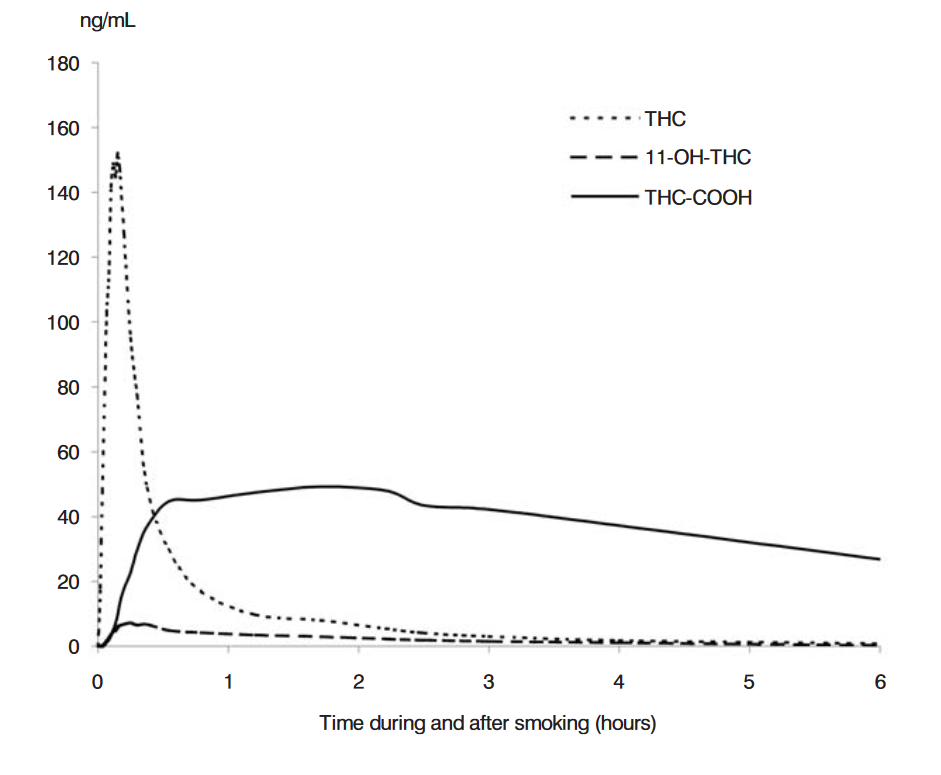
\includegraphics[height=10cm]{THCKonzentration}
		\captionsetup{font=small}
		\captionof{figure}{Entwicklung der THC Konzentration im Blut}
		\small 
		\noindent
		\begin{center}
		Quelle: \cite{giroud}
		\end{center}
	 }	
	 
	 \noindent \\
	 Mit einer Legalisierung sollte ein Grenzwert in Betracht gezogen werden.
	 Der Grenzwert sollte sich am bereits bestehenden Alkoholgrenzwert von 0.5 Promille orientieren. 
	 Vor allem sinnvoll wäre dieser Grenzwert für regelmässige Konsumenten, bei denen der Wert nur langsam sinkt.
	 Mit der neuen Regelung wären regelmässige Konsumenten bereits nach mehreren Stunden rechtlich wieder fahrfähig.
	 
	 
	 \subsection{Besteuerung}
	 Durch die Legalisierung und neue Rechtslage besteht die Möglichkeit, dass Cannabis besteuert werden kann.
	 Der Staat kann mehr Einnahmen für die Staatskasse generieren und den Marktpreis direkt beeinflussen.
	 Erhöhte Steuern würden sich direkt im Marktpreis wiederspiegeln.
	 Die Besteuerung erfolgt auf verschiedenen Stufen und indirekte Steuern werden auch berücksichtigt.
	 
	 \paragraph{Mehrwertsteuer}
	 Die Mehrwertsteuer ist eine universelle Steuer und wird auf den Bruttoverkaufspreis erhoben.
	 Sie ist im Bundesgesetz über die Mehrwertsteuer (MWSTG) geregelt.
	 Nach \texttt{Art. 25 Abs. 1 MWSTG} beträgt der Normalsatz 7.7\% und der reduzierte Satz 2.5\%.
	 Für den grössten Teil des Marktvolumens gilt der Normalsteuersatz, da wir von THC-haltigem Cannabis ausgehen, das rein zum Freizeitkonsum dient und keinerlei medizinische Zwecke hat. 
	 Der Anteil der medizinischen Anwendungen von THC ist noch so klein, dass man ihn vernachlässigen kann.
	 Das im Kapitel \texttt{Legalisierung > Preisniveau} besprochene Preisniveau bezieht sich auf den Bruttoverkaufspreis, den die Konsumenten bezahlen.
	 Die Mehrwertsteuer ist jedoch schon im Bruttoverkaufspreis von CHF 11.50 enthalten.
	 Man schliesst so daraus, dass der Nettoverkaufspreis CHF 10.68 und die Mehrwertsteuer CHF 0.82 CHF pro Gramm beträgt.\\
	 
	 \noindent
	 Für die Berechnung wird das im Kapitel 2.4 ermittelte höhere Marktvolumen von 54.7 Tonnen verwendet.	 
	 Die durch den Staat eingenommene Mehrwertsteuer wird so auf CHF 15'316'000 geschätzt.
	 	 
	 
	 \paragraph{Cannabissteuer}
	 Durch eine gezielte Steuer kann der Staat die Nachfrage von Cannabis steuern. 
	 Es ist eine Sache von Präferenz, ob man eine einfache oder aggressive Besteuerungsstrategie nehmen möchte.
	 Man kann die Besteuerung auch zusätzlich mit einer Lizenzierungspflicht kombinieren.
	 Das erzielte Einkommen aus der Cannabissteuer ist vom Steuersatz abhängig und kann noch nicht berechnet werden.
	 Da der Steuersatz variieren kann, wird in dieser Arbeit nur der maximale Steuersatz berechnet.\\
	 
	 \noindent
	 Der Vorverkaufpreis von einem Gramm Cannabis wird etwa auf CHF 6.17 geschätzt \cite{bandli}.
	 Mit der Mehrwertsteuer von CHF 0.82 einberechnet ergibt sich dann ein Besteuerungsspielraum von CHF 4.51 pro Gramm.
	 Dies ergibt ein maximales Gesamtsteueraufkommen der Cannabissteuer von CHF 246'697'000.
	 
	 
	 \paragraph{Andere Besteuerungsarten}
	 Eine Legalisierung würde dem Staat weitere Einnahmen in Form von Gewinnsteuer und Einkommensteuer bringen.
	 Diese Werte sind jedoch nicht für die Zukunft zu berechnen, da der Markt stark schwanken kann.
	 Desweiteren würden die Angestellten der Unternehmen ihre AHV / IV Beiträge bezahlen.
	 
	 

\end{document}